% arara: xelatex: { shell: yes, synctex: yes }
\RequirePackage[l2tabu, orthodox]{nag}
\documentclass[english,fira]{ist-report}

% -- Texto e codificação
\usepackage{anyfontsize}
\usepackage{pdflscape}



% -- Símbolos extra
\usepackage{amssymb}
\usepackage{textcomp}
\usepackage{gensymb}
\usepackage{cancel}

% -- Redefine margins
\geometry{top = 1cm}

% -- Bibliografia
\usepackage[
	backend = biber,
	style = alphabetic,
	sorting = ynt,
	%alldates=iso
	]{biblatex}
\usepackage{fvextra}
\usepackage{csquotes}

% --  Definições de imagens
\graphicspath{{graphics/}}
\usepackage{caption}
\usepackage{subcaption}
\usepackage{afterpage}
\usepackage{tabularx}

% -- Desenhar circuitos elétricos e lógicos
\usepackage{tikz}
\usepackage{pgfplots}
\usepackage{circuitikz}
\usetikzlibrary{arrows.meta,positioning,patterns,graphs}
\pgfplotsset{compat=1.15}
\pgfplotsset{table/search path = {data}}
\pgfplotsset{/pgf/number format/use comma,}

% -- Integrar código fonte
\usepackage{minted}
\usepackage{verbatim}
\usepackage{algorithm}
\usepackage{algpseudocode}

% -- Tabelas
\usepackage{booktabs}
\usepackage{makecell}

% -- Misc
\usepackage[disable]{todonotes}

% -- Funções matemáticas extra
\usepackage{siunitx}
\sisetup{
  math-ohm=\Omega,
  text-ohm=\ensuremath{\Omega},
}

\title{Distributed Real-Time Control Systems}

% TikZ and minted hotfix, cuz those are fun
\makeatletter
\global\let\tikz@ensure@dollar@catcode=\relax
\makeatother

%\definecolor{codebg}{rgb}{0.97,0.97,0.97}
%\setminted[c]{bgcolor = codebg, breaklines, linenos}
%\setmintedinline[c]{bgcolor = {}}

\setminted[c]{linenos, frame = leftline, breaklines}

\newrobustcmd*{\matr}[1]{\symbf{#1}}
\newrobustcmd*{\ccode}[1]{\mintinline{c}{#1}}

\newrobustcmd*{\ccheckmark}{\tikz\fill[scale=0.4](0,.35) -- (.25,0) -- (1,.7) -- (.25,.15) -- cycle;} 

\renewcommand{\baselinestretch}{1.15}

\addbibresource{bibliography.bib}

\begin{document}

\begin{titlepage}

\begin{center}
	\vspace*{0.1\textheight}
	
\includegraphics[width = 0.4\linewidth, trim = {172.4pt 202.7pt 172.6pt 201.4pt}, clip]{IST_A_CMYK_POS}
	
	\vspace*{0.1\textheight}
	{\huge\bfseries Real-Time Cooperative Decentralized Control of a Smart Office Illumination System}
	
	\vspace*{0.03\textheight}
	{\Large Distributed Real-Time Control Systems Final Project}
	
	\vspace*{43.5mm}
	{\Large \begin{tabular}{l r} Daniel de Schiffart & \texttt{81479} \\ João Gonçalves & \texttt{81040} \\ Francisco Castro & \texttt{78655}\end{tabular}}
	
	\vspace{\fill}
	{\large Distributed Real-Time Control Systems}
	
	\vspace*{0.01\textheight}
	{\Large Master's Degree in Aerospace Engineering}
	
	\vspace*{0.01\textheight}
	{\large Instituto Superior Técnico}
\end{center}

\end{titlepage}
\setcounter{page}{1}

\begin{abstract}
	In this technical report we will present the design and development of a LED-powered office illumination system that implements distributed real-time control to maintain comfortable levels of luminance for its users. We will discuss the approaches done to the modelling of each sensor and corresponding LED and its individual control system, the method of communication between all connected sensor-LED pairs (henceforth referred to as desks), the interaction between the lights emitted by each desk and their joined effort to reduce lighting costs and maximize user comfort, and the gathering of relevant data for diagnostics.
\end{abstract}

{\hypersetup{linkcolor = black} \tableofcontents}

\section{Introduction}




\pagebreak
\appendix

\todo[inline]{Mencionar que toda a implementação é feita para 2 nodes, apesar de ser tudo extensível, blah blah}

\section{Report Structure}

This should be the report structure according to the class slides (Distributed Real-Time Control Systems, module 32).
\begin{description}
	\item[Abstract] A summary in less than 200 words;
	\item[Introduction] Motivation, challenges, main idea, objectives, outline;
	\item[Background/Concepts] Common knowledge required;
	\item[Related Work] State-of-the-art;\todo[inline]{I vote for self driving cars}
	\item[Development] Your approach, methodologies, innovations;
	\item[Experiments] Carefully explain the design of the experiments;
	\item[Results] Illustrate and comment on the results of experiments;
	\item[Discussion] Maybe in results;
	\item[Conclusions and Future] Critically comment on what was achieved and indicate points of improvement;
	\item[Bibliography]
	\item[Appendices]
\end{description}

Report should be less than 20 pages total, including everything.

\subsection{Discussable Topics}

\begin{itemize}
	\item Theoretical introduction and discussion of topic (office space illumination)
	\item Objective
	\item Composition of desks
	\item Illuminance measurement system
	\item LED actuation system
	\item Desk illumination model
	\item Desk illumination controller
	\item Gathering data
	\item Inter-desk communication
	\item Bus monitoring
	\item Calibration
	\item Distributed control algorithm
	\item Data server
	\begin{itemize}
		\item Performance metrics
		\item C++ implementation
	\end{itemize}
\end{itemize}

Implementation notes from stage 1.
\begin{itemize}
	\item Make plots for the different signals in the control system (references, control values, measurements) and compute metrics that show the correct operation of the system.
	\item Choose messages with short size and a high baud rate. Compute communication delays and verify that the communication time can be acommodated within the available control loop period.
	\item Graphically visualize the data in MATLAB or Excel.
\end{itemize}

Documentation notes from stage 1.
\begin{itemize}
	\item Take pictures of the interior and of the exterior of the box enclosing the luminaires. Make sure that you illustrate the position of the LED, the LDR and the emission/reflection path.
	\item Show plots of the steady state characteristic of the system. Show step responses of the system in different illuminance conditions.
	\item Characterize the jitter in your control system. How much does the sampling rate deviate from the desired one?
	\item Characterize the error in your feedforward controller. In particular, implement a predictor of your system and compute the average mean squared error between the prediction and the measurements.
	\item Characterize the dynamic characteristics of the feedback controller, in different illuminance conditions (overshoot, damping factor).
	\item Illustrate any improvements that you make to the basic feedback controller (feedforward term, anti-windup, etc) with plots of the time responses.
	\item Comment the Arduino code for your controller.
	\item Characterize the processing time taken by the control computation, serial communications and other computations.
\end{itemize}

Documentation notes from stage 2. \\
\textit{``In your report, please do not forget to address the following issues''}
\begin{description}
	\item[I2C communications] Indicate the average time required to send a request message and receive an answer.
	\item[C++ classes, sockets, parallelism] Indicate the C++ classes that are most relevant for coding the server running on the PC interfacing to the Arduinos.
	\item[Sockets] List the number of sockets used to implement the server. Describe the functions of the sockets.
	\item[Concurrency] Indicate the methodologies used in the server to implement parallelism in order to process requests from multiple clients.
	\item[Distributed control] Describe the implementation of the cooperative distributed controller.
	\item[Experiments] Perform experiments to compare results between the cooperative distributed contrller and the non-cooperative controller (independent local controllers). Plot the time response of both controllers in similar situations and create a table with their performance metrics.
\end{description}


\section{Raspbian Startup}
\begin{enumerate}
	\item Open console
	\item \texttt{sudo ifconfig enp2s0f0 10.0.0.2 netmask 255.255.255.0}
	\item Configure by hand on Ubuntu wired connection settings
	\begin{enumerate}
		\item Details -> Disable \textit{Connect Automatically}
		\item IPv4 -> \textit{IPv4 Method} to \textit{Manual}
		\item Set address to \texttt{10.0.0.2} and gateway to \texttt{255.255.255.0}
	\end{enumerate}
	\item Run \texttt{ssh pi\@10.0.0.1} and use \texttt{raspberry} as password
\end{enumerate}

\paragraph{Importante} Antes de desligar o Raspberry Pi, correr \texttt{sudo shutdown -h now} para evitar corrupção do sistema operativo.

\section{Illumination system calibration}

\subsection{Principles of the calibration procedure}

The illuminance at each desk follows the model
\begin{gather}
  L = K \matr{d} + \matr{o} \nonumber \\ 
  \left[\begin{array}{c} l_{1}\\ l_{2} \end{array}\right] =
  \left[\begin{array}{cc}
	k_{11} & k_{12}\\
	k_{21} & k_{22}
  \end{array}\right]
  \left[\begin{array}{c} d_{1}\\ d_{2}\end{array}\right]+
  \left[\begin{array}{c} o_{1}\\ o_{2} \end{array}\right]
  \label{eq:model}
\end{gather}
where $l_i$, $d_i$ and $o_i$ are the illuminance, LED power (in percentage) and background illuminance at desk $i$, respectively. The purpose of the calibration is to find the values for $k_{ij}$ and $o_i$ for a given office layout.

The calibration is performed by turning the lumiaires synchronously and taking measurements. One node takes initiative and sends a message to trigger the process. First, both LEDs are switched off and $o_i$ is measured.
Then, node 2 turns on its LED, measures the resulting illuminance and computes $k_{22}$, and sends the illuminance to node 1. Receiving this value, node 1 can also measure its illuminance and compute $k_{21}$. The operation inverts and $k_{12}$ and $k_{11}$ are determined. In the end, nodes share the results.

\subsection{Implementation detais}

The previous procedure is implemented as its own module, with a special communication protocol. The flow chart in figure \ref{fig:calib} illustrates messages sent and summarizes the finite-state machine.
Between changing the LED state and taking measurements, the nodes must sleep, to guarantee that the measurement is taken in steady state. For this, they were set to sleep for a lenght of time 10 times the value of the system time constant, $10 \times \SI{5}{\milli \second} = \SI{50}{\milli \second}$. 

It also should be noted that internally, the nodes are not distinguishable as 1 and 2. Each considers itself node 1 and the peer as 2, so the representation of the coupling matrix $K$ is transposed by both diagonals, and identically $o_1$ and $o_2$ are swapped.

\section{Optimização do Sistema Distribuído}

\begin{gather*}
	u^* = \text{argmin}\,J(x, \mu) \\
	l_i = \sum^n_{j=1} d_j k_{ij} + o_i \geq L_i, \qquad 0 \leq d_i \leq 100, \quad \forall i \\
	\matr{l} = \matr{K}\matr{d} + \matr{o} \geq \matr{L}, \qquad 0 \leq d \leq 100
\end{gather*}
Se as condições aqui listadas não forem cumpridas, o problema é declarado \textit{unfeasible}. A função de custo é
\begin{gather*}
	f(d) = c_1d_1 + c_2d_2 + \ldots + c_nd_n = \matr{C}^T\matr{d}
\end{gather*}
onde $\matr{c}$ é o vetor dos custos de energia.

Ver os cantos do domínio admissível e saber o ponto com menor custo. Assim, obtém-se $(d_1,d_2)$. Mais à frente adicionamos maximização de longevidade de lâmpadas.
\begin{figure}[ht]
	\centering
	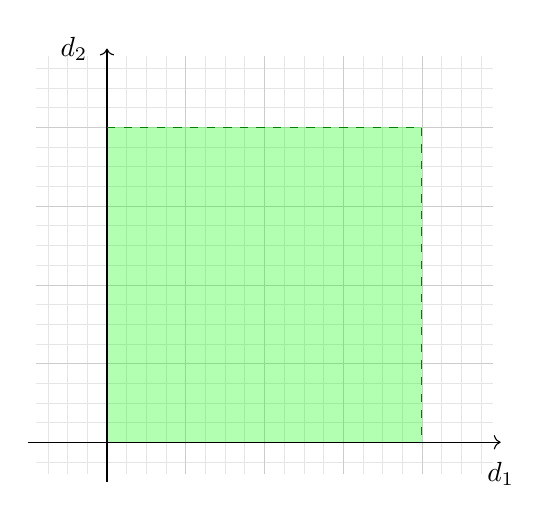
\begin{tikzpicture}
	\coordinate (axis) at (0,0);
	\node at (0,5) [label={180:$d_2$}] {};
	\node at (5,0) [label={-90:$d_1$}] {};
	\draw [step=0.25,draw=black!10!white,very thin] (-0.9,-0.4) grid (4.9,4.9);
	\draw [step=1,draw=black!20!white,very thin] (-0.9,-0.4) grid (4.9,4.9);
	\fill [fill=green,opacity=0.3] (0,0) -- (0,4) -- (4,4) -- (4,0) -- cycle;
	\draw [->] (axis) ++(0,-0.5) -- (0,5);
	\draw [->] (axis) ++(-1,0) -- (5,0);
	\draw [dashed,color={green!50!black}] (axis) (0,4) -- (4,4) -- (4,0);
\end{tikzpicture}

	\caption{Admissible domain and dimming value selection.}
\end{figure}

\section{Arduino data fomat}

{\centering \textit{Provisory section so that Daniel can start the web-server}}

Each Arduino sends data at every sample time so that the server can store the necessary information. 

A message is designed to be a fixed-size word, with the least number of bits possible.
Currently, the message has 20 bytes, as seen in this segment from \texttt{comms.h}:
%\todo[inline]{Minted com xelatex exibe as tabs como \texttt{^^I}. E os underscores, se não fizer escape dão erros com o Tikz.}
\begin{minted}[firstnumber = 20]{c}
typedef struct msg{
    MsgCode code; // 1 byte
    uint8_t address; // 1 byte
    uint8_t aux1; // 1 byte
    uint8_t aux2; // 1 byte
    float value[4]; // 4 x 4 = 16 bytes

}message_t; //size fixed to 20 bytes
\end{minted}

\ccode{code} is an unsigned integer (\ccode{uint8_t}) which represents what the data format is.
Some values for this are used in the callibration procedure, but the value for sample time data forwarding is, for now, 5.
A way of knowing this every time is having the same \ccode{enum} in the server as in the Arduino \texttt{comms} module:
\begin{minted}[firstnumber = 9]{c}
enum MsgCode : uint8_t{

    calibration_request,
    data,
    cont,
    acknowledge,
    consensus_data,
    sampling_time_data,

};
\end{minted}

The rest of the data is:
\begin{table}[ht]
	\centering
	\begin{tabular}[h]{l|l}\toprule
		\ccode{address} & Arduino's I$2$C address. \\
		\ccode{aux1}    & 1st MSB: Desk occupancy state ($1$ for occupied, $0$ for free). \\
		                & next 7 bits, led duty cycle, unsigned integer from $0$ to $100$. \\
		\ccode{aux2}    & Illuminance lower bound (presumably $40$ or $80$), in LUX. \\
		\ccode{value[0]}& Measured illuminance, in LUX. \\
		\ccode{value[1]}& Local background illuminance, in LUX. \\
		\ccode{value[2]}& Instantaneous control illuminance reference, in LUX. \\
		\ccode{value[3]}& Instantaneous power consumption, units to be defined. \\
		\bottomrule
	\end{tabular}
\end{table}

Note, to extract the duty cycle and occupancy state, you can do:
\begin{minted}[linenos=false,frame=none]{c}
  unsigned duty_cycle = aux1 & (0x7F); // This is a bit-wise and with 0111111
  bool state = aux1 & (0x80); // This is a bit-wise and with 10000000 
\end{minted}

From what I see, this is everything we need to send the server, and it should be able to compute the necessary variables. The following table should summarize my thoughts:
\begin{table}[h]
	\centering
	\begin{tabularx}{\linewidth}{l|X}
		Quantity & How to determine (\ccheckmark{} means it is sent every sample time) \\
		Illuminance & \ccheckmark{} \\
		duty cycle  & \ccheckmark{} \\
		occupancy state & \ccheckmark{} \\
		lower bound & \ccheckmark{} \\
		Control reference & \ccheckmark{} \\
		Background illuminance & \ccheckmark{} \\
		Instantaneous power consumption & \ccheckmark{} \\
		Total power consumption & Sum of instantaneous power consumption for all nodes. \\
		Time since last restart & listen to a specific message code (to be defined) and keep the timestamp. \\
		Node energy spent since last restart & integrate node's instantaneous power consumption, sample time is fixed and known. \\
		Total energy since last restart & Sum both nodes's energy spent. \\
		Node confort error since last restart & At each sample time we have the lower bound and the illuminance, do the math. \\
		Total confort error since last restart & Sum both nodes' confort error. \\
		Node flicker since last restart & See project description, all that is needed is the illuminance from the last 3 samples. \\
		Total flicker since last restart & Sum both nodes' flicker.
	\end{tabularx}
\end{table}

I might have missed something, we'll see.

\section{Schematics and Charts}

\begin{figure}[ht]
	\centering
	\begin{tikzpicture}
	\tikzstyle{arduino} = [draw,minimum height=80,inner sep=30];
	\tikzstyle{wire} = [];
	\node at (0,0) (ard1) [arduino] {\Large Arduino 1};
	\node (ard2) [right=4cm of ard1,arduino] {\Large Arduino 2};
	\node (rpi) [above=2cm of ard2,arduino] {\Large Raspberry Pi};
	\path (ard1.north east) to node (ard1_scl) [auto, swap, align=right] {\ttfamily SCL} ++(0,-3);
	\path (ard1.north east) to node (ard1_sda) [auto, swap, align=right] {\ttfamily SDA} ++(0,-4);
	\path (ard1.north east) to node (ard1_gnd) [auto, swap, align=right] {\ttfamily GND} ++(0,-5);
	\path (ard2.north west) to node (ard2_scl) [auto, align=left] {\ttfamily SCL} ++(0,-3);
	\path (ard2.north west) to node (ard2_sda) [auto, align=left] {\ttfamily SDA} ++(0,-4);
	\path (ard2.north west) to node (ard2_gnd) [auto, align=left] {\ttfamily GND} ++(0,-5);
	\path (rpi.north west) to node (rpi_19) [auto, align=left] {\ttfamily 19} ++(0,-3);
	\path (rpi.north west) to node (rpi_18) [auto, align=left] {\ttfamily 18} ++(0,-4);
	\path (rpi.north west) to node (rpi_gnd) [auto, align=left] {\ttfamily GND} ++(0,-5);
	\draw (ard1_scl) -- (ard2_scl) (ard1_sda) -- (ard2_sda) (ard1_gnd) -- (ard2_gnd);
	\path (ard1_scl) ++(1.7,0) coordinate (coord1);
	\path (ard1_sda) ++(2.4,0) coordinate (coord2);
	\path (ard1_gnd) ++(3.1,0) coordinate (coord3);
	\draw (coord1) to [short,*-,R] (coord1 |- rpi_19) to [short,-] (rpi_19.west);
	\draw (coord2) to [short,*-,R] (coord2 |- rpi_18) to [short,-] (rpi_18.west);
	\draw (coord3) to [short,*-] (coord3 |- rpi_gnd) to [short,-] (rpi_gnd.west);
\end{tikzpicture}

	\caption{Arduino and Raspberry Pi setup.}
\end{figure}

\begin{figure}[ht]
	\centering
	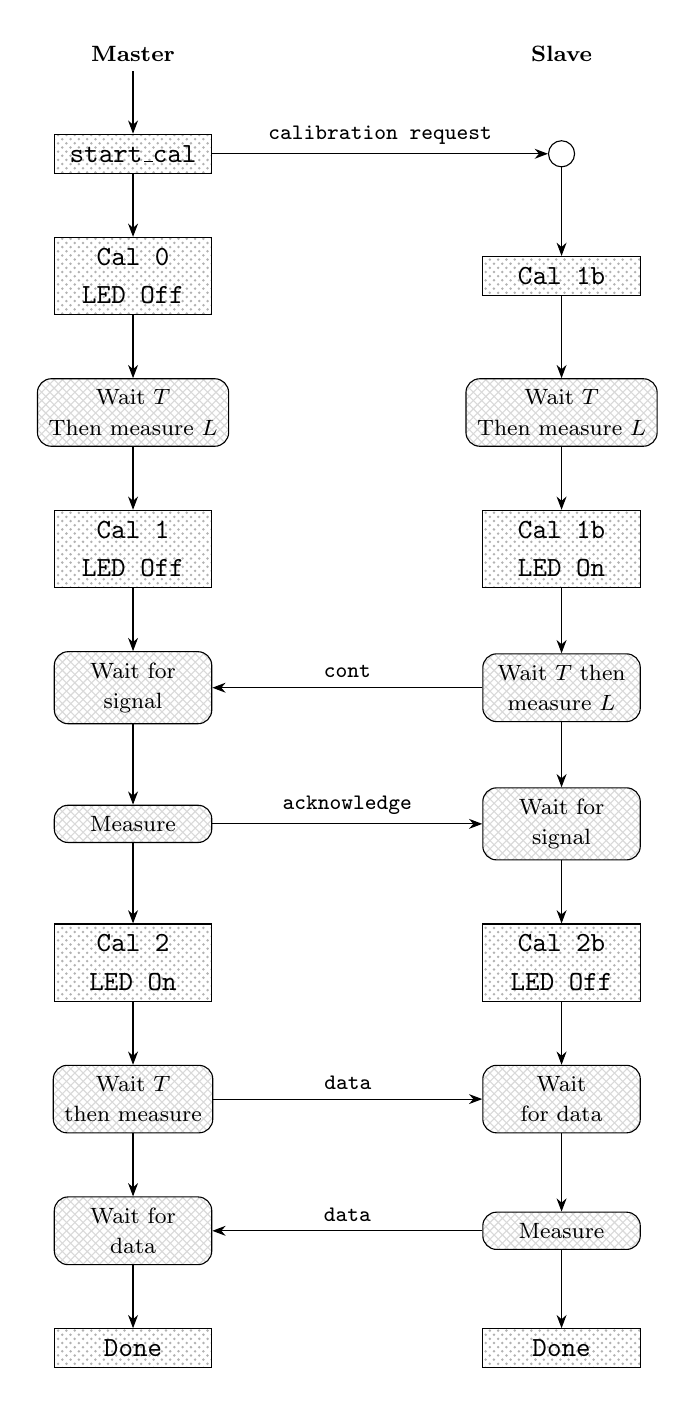
\begin{tikzpicture}
	\tikzstyle{every node}=[font=\footnotesize];
	\tikzstyle{stt}=[draw,rectangle,align=center,inner sep=4pt,minimum width=20mm,fill,pattern=crosshatch dots,pattern color=black!30!white,font=\ttfamily];
	\tikzstyle{stp}=[draw,rectangle,align=center,inner sep=4pt,minimum width=20mm,rounded corners=5pt,fill,pattern=crosshatch,pattern color=black!15!white];
	\tikzstyle{pth}=[draw,->,thick];
	\matrix[row sep=8mm,column sep=3cm]{
		\node (master_start) [] {\textbf{Master}};			& \node (slave_start) [] {\textbf{Slave}};			\\
		\node (m1) [stt] {start\_cal};						& \node (s1) [circle, draw] {};						\\
		\node (m2) [stt] {Cal 0 \\ LED Off};				& \node (s2) [stt] {Cal 1b};						\\
		\node (m3) [stp] {Wait $T$ \\ Then measure $L$};	& \node (s3) [stp] {Wait $T$ \\ Then measure $L$};	\\
		\node (m4) [stt] {Cal 1 \\ LED Off};				& \node (s4) [stt] {Cal 1b \\ LED On};				\\
		\node (m5) [stp] {Wait for \\ signal};				& \node (s5) [stp] {Wait $T$ then \\ measure $L$};	\\
		\node (m6) [stp] {Measure};							& \node (s6) [stp] {Wait for \\ signal};			\\
		\node (m7) [stt] {Cal 2 \\ LED On};					& \node (s7) [stt] {Cal 2b \\ LED Off};				\\
		\node (m8) [stp] {Wait $T$ \\ then measure};		& \node (s8) [stp] {Wait \\ for data};				\\
		\node (m9) [stp] {Wait for \\ data};				& \node (s9) [stp] {Measure};						\\
		\node (master_end) [stt] {Done};					& \node (slave_end) [stt] {Done};					\\
	};
	\graph [use existing nodes,edges=-{Stealth[]}]{
		master_start -> m1 -> m2 -> m3 -> m4 -> m5 -> m6 -> m7 -> m8 -> m9 -> master_end;
		s1 -> s2 -> s3 -> s4 -> s5 -> s6 -> s7 -> s8 -> s9 -> slave_end;
		m1 -> [edge node={node[font=\footnotesize\ttfamily,auto]{calibration request}}] s1;
		s5 -> [edge node={node[font=\footnotesize\ttfamily,auto,swap]{cont}}] m5;
		m6 -> [edge node={node[font=\footnotesize\ttfamily,auto]{acknowledge}}] s6;
		m8 -> [edge node={node[font=\footnotesize\ttfamily,auto]{data}}] s8;
		s9 -> [edge node={node[font=\footnotesize\ttfamily,auto,swap]{data}}] m9;
	};
\end{tikzpicture}

	\caption{Calibration procedure. Used $T$=\SI{0.5}{\second}.}
	\label{fig:calib}
\end{figure}

\pagebreak
\printbibliography

\listoftodos
\end{document}
